% !TEX program = xelatex
% Compile:  latexmk -xelatex main.tex      (biber runs automatically)
% Options:  lang=zh|en  font=newcm|libertinus|stix  review  numbering=section  paper=letter
% Chinese spacing tip: \cref / \textcite output behaves like a Latin word. Put a space on the
% side where it ends in a digit or Latin letter (\cref{tab:x} 给出), none where it touches CJK
% (由\cref{eq:x} 及, 可参考\textcite{chen1999advanced}).
\documentclass[lang=zh]{mainsub-report}

\addbibresource{references.bib}

\title{岭回归中的偏差—方差权衡}
\subtitle{一份模板演示：数学、图表、代码与交叉引用}
\author{Mainsub}
\affiliation{中国科学技术大学}
\date{\today}
\shorttitle{岭回归中的偏差—方差权衡}
\keywords{岭回归；偏差—方差分解；收缩估计}

\begin{abstract}
本文以岭回归为例演示模板的排版效果。我们在高斯线性模型下推导岭估计量的偏差与方差，
说明适度的收缩如何以少量偏差换取方差的显著下降，并用一个模拟实验验证这一结论。
\end{abstract}

\begin{document}
\maketitle

\section{引言}

当设计矩阵 $X$ 的列高度相关时，最小二乘估计 $\hat\beta = (X^\top X)^{-1}X^\top y$ 的方差会急剧膨胀。
\textcite{hoerl1970ridge} 提出在 $X^\top X$ 的对角线上加入一个正常数，以\emph{牺牲无偏性为代价}换取更稳定的估计；
这一思想后来成为收缩估计（shrinkage estimation）的基石\parencite{hastie2009elements}。
关于线性模型的经典理论，可参考\textcite{chen1999advanced}。\footnote{本文所有数值结果均可由附录中的代码复现。}

本文的结构如下：\cref{sec:model}给出模型与估计量，\cref{sec:sim}给出数值示例。

\section{模型与估计量}\label{sec:model}

\subsection{设定}

\begin{assumption}[高斯线性模型]\label{asm:gauss}
观测满足 $y = X\beta + \eps$，其中 $X\in\R^{n\times p}$ 为固定设计，$\eps \sim \Normal(0, \sigma^2 I_n)$。
\end{assumption}

\begin{definition}[岭估计量]\label{def:ridge}
对给定的 $\lambda > 0$，岭估计量定义为
\begin{equation}\label{eq:ridge}
  \hat\beta_\lambda
  = \argmin_{b\in\R^p} \Bigl\{ \norm{y - Xb}_2^2 + \lambda \norm{b}_2^2 \Bigr\}
  = (X^\top X + \lambda I_p)^{-1} X^\top y .
\end{equation}
\end{definition}

\subsection{偏差与方差}

记 $X = UDV^\top$ 为奇异值分解，$d_1\ge\cdots\ge d_p>0$ 为奇异值。

\begin{proposition}\label{prop:bv}
在\cref{asm:gauss} 下，岭估计量的偏差与协方差分别为
\begin{align}
  \Bias(\hat\beta_\lambda) &= -\lambda\,(X^\top X + \lambda I_p)^{-1}\beta, \label{eq:bias}\\
  \Var(\hat\beta_\lambda)  &= \sigma^2 \sum_{j=1}^{p} \frac{d_j^2}{(d_j^2+\lambda)^2}\, v_j v_j^\top . \label{eq:var}
\end{align}
因此 $\tr\Var(\hat\beta_\lambda)$ 关于 $\lambda$ 严格递减，而当 $\beta\neq0$ 时 $\norm{\Bias(\hat\beta_\lambda)}_2^2$ 严格递增。
\end{proposition}

\begin{proof}
由\cref{eq:ridge} 及 $\E y = X\beta$ 得 $\E\hat\beta_\lambda = (X^\top X+\lambda I)^{-1}X^\top X\beta$，
两边减去 $\beta$ 即得\cref{eq:bias}。又 $\Var(y)=\sigma^2 I_n$，代入奇异值分解
$(X^\top X+\lambda I)^{-1}X^\top = V\diag\bigl(d_j/(d_j^2+\lambda)\bigr)U^\top$ 即得\cref{eq:var}。
\end{proof}

\begin{remark}
当 $\lambda\to0$ 时 $\hat\beta_\lambda$ 收敛到最小二乘估计；当 $\lambda\to\infty$ 时 $\hat\beta_\lambda\to0$。
均方误差 $\MSE(\lambda) = \norm{\Bias}_2^2 + \tr\Var$ 在两者之间取得最小值。
\end{remark}

\section{数值示例}\label{sec:sim}

我们取 $n=120$、$p=6$，设计矩阵的行独立服从 $\Normal(0,\Sigma)$，其中 $\Sigma_{ij}=0.6^{\abs{i-j}}$，
真实系数 $\beta=(2,-1.5,1,0,0,0.5)^\top$，$\sigma=2$。\cref{fig:path} 给出系数随 $\lambda$ 的收缩路径，
\cref{tab:mse} 给出由\cref{eq:bias,eq:var} 精确计算的风险分解。

\begin{figure}[htbp]
  \centering
  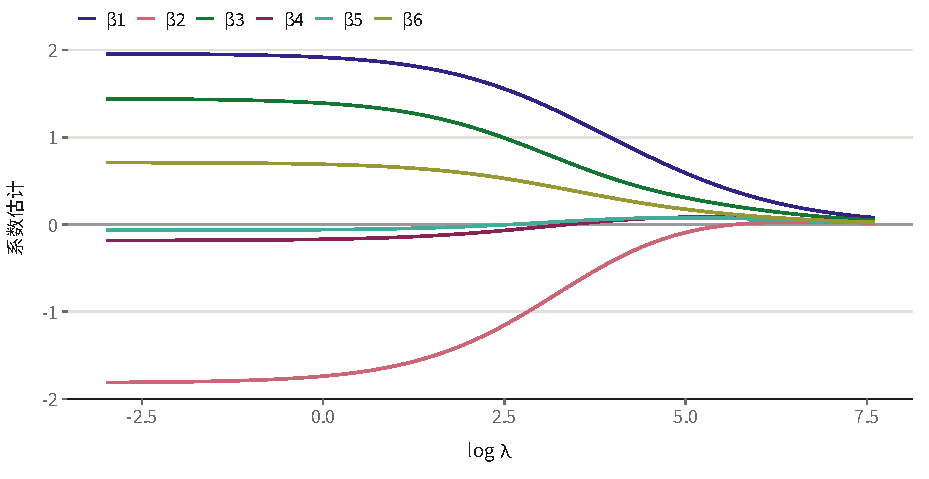
\includegraphics[width=\linewidth]{figures/ridge-path.pdf}
  \caption{岭回归的系数路径。随着 $\lambda$ 增大，所有系数被连续地压向零。}
  \label{fig:path}
\end{figure}

\begin{table}[htbp]
  \centering
  \caption{不同 $\lambda$ 下的偏差、方差与均方误差}
  \label{tab:mse}
  \begin{tabular}{@{}rrrr@{}}
    \toprule
    $\lambda$ & $\norm{\Bias}_2^2$ & $\tr\Var$ & $\MSE$ \\
    \midrule
    0   & 0.000 & 0.449 & 0.449 \\
    1   & 0.008 & 0.424 & 0.432 \\
    2   & 0.029 & 0.402 & \textbf{0.430} \\
    5   & 0.148 & 0.345 & 0.493 \\
    20  & 1.110 & 0.195 & 1.305 \\
    100 & 4.030 & 0.048 & 4.078 \\
    \bottomrule
  \end{tabular}
\end{table}

从\cref{tab:mse} 可以读出三点：
\begin{enumerate}
  \item 方差随 $\lambda$ 单调下降，偏差单调上升，与\cref{prop:bv} 一致；
  \item 在 $\lambda = 2$ 附近，MSE 低于最小二乘（$\lambda=0$）；
  \item 过度收缩（$\lambda=100$）使偏差主导风险。
\end{enumerate}

计算岭估计量只需要一行线性代数：
\begin{lstlisting}[language=R]
ridge <- function(X, y, lambda) {
  p <- ncol(X)
  solve(crossprod(X) + lambda * diag(p), crossprod(X, y))  # 求解正规方程
}
\end{lstlisting}

\section{结论}

岭回归说明了统计学中一个反复出现的主题：\emph{无偏并不等于好}。在实践中，$\lambda$ 通常由交叉验证选取。

\printbibliography

\appendix
\section{补充推导}\label{app:extra}

在正交设计 $X^\top X = I_p$ 下，岭估计量是最小二乘估计的简单缩放：
\[
  \hat\beta_\lambda = \frac{1}{1+\lambda}\,\hat\beta^{\mathrm{OLS}},
  \qquad
  \MSE(\lambda) = \frac{p\,\sigma^2 + \lambda^2\norm{\beta}_2^2}{(1+\lambda)^2},
\]
其最小值在 $\lambda^\star = p\sigma^2/\norm{\beta}_2^2$ 处取得。

\end{document}
